\documentclass[11pt,a4paper]{article}
\usepackage[T1]{fontenc}\usepackage[utf8]{inputenc}
\usepackage{amsmath,amssymb,amsthm,mathtools,graphicx,booktabs,multirow,array}
\usepackage[font=small]{caption}
\graphicspath{{figures/}}
\usepackage{xcolor}\usepackage[colorlinks=true]{hyperref}\usepackage{url}
\usepackage{tikz}
\usetikzlibrary{arrows.meta,positioning,shapes.geometric,fit,calc}
\newcommand{\CBSLAO}{\textsc{CBSLAO}}
\newcommand{\CBUC}{\textsc{CBUC}}
\newcommand{\BwK}{\textsc{BwK}}
\newcommand{\ReAct}{\textsc{ReAct}}
\newcommand{\Oh}{\mathcal{O}}
\newcommand{\tOh}{\widetilde{\mathcal{O}}}
\newcommand{\Ex}{\mathbb{E}}
\newcommand{\Prob}{\mathbb{P}}
\DeclareMathOperator*{\argmax}{arg\,max}
\newtheorem{theorem}{Theorem}\newtheorem{lemma}{Lemma}
\newtheorem{remark}{Remark}\newtheorem{proposition}{Proposition}
\newtheorem{corollary}{Corollary}\newtheorem{definition}{Definition}
\begin{document}
\section{\CBUC\ (excerpt)}
\input{/tmp/algo_new.tex}
\section{Evaluation}
\label{sec:evaluation}

\subsection{Research questions}
\begin{description}
  \item[E-RQ1.] How often do existing LLM-agent controllers violate
    user-declared budgets and deadlines on realistic workloads?
  \item[E-RQ2.] Does \CBUC~reduce violation rate, and at what utility
    cost?
  \item[E-RQ3.] How does \CBUC's advantage scale with tool-pool size
    $K$, budget tightness $\rho$, and cost-tail heaviness?
\end{description}

\subsection{Simulator and workloads}
We implement a deterministic-seed simulator \texttt{cbslao\_sim.py}
(released) with pluggable cost/latency/utility distributions. The
current study is a \emph{controlled synthetic simulation}; replication
on real LLM API traces is future work
(\S\ref{sec:threats}). The sweep grid is
\[
  K \in \{10, 50, 200\},\quad
  \rho = \tfrac{B}{\sum_i \Ex[c_i]}
      \in \{0.2, 0.5, 1.0\},\quad
  \alpha \in \{1.5, 2.5\},\quad
  n = 30\text{ seeds/cell}.
\]
The headline extended sweep uses $n=20$ seeds per workload cell. This
gives $18$ workload cells and $360$ runs per policy; with $11$
policies, Table~\ref{tab:headline} contains $3{,}960$ replicate rows.
Costs are Pareto, latencies Gaussian, utilities Gaussian-clipped.
Aggregate utility uses a saturating aggregator
$U(h) = 1 - \exp(-\sum_i u_i)$ to reflect diminishing returns of
redundant tool calls.

\subsection{Baselines and \CBUC~variants}
We deliberately include four \emph{constraint-aware} baselines
(Lagrangian, CVaR-\BwK, pre-check UCB, and the non-adaptive
chance-constrained knapsack oracle) in addition to the status-quo
agent-loop proxies (\ReAct-uncapped, \ReAct-capped), so that any
improvement from \CBUC~cannot be attributed to a strawman comparison.

\begin{enumerate}
  \item \ReAct-uncapped: myopic greedy ignoring budget (realistic for
    default agent loops).
  \item \ReAct-capped: stops once realised cost exceeds budget
    (soft-prompt analog).
  \item Non-adaptive greedy: offline ranking by the true
    $\mu_i / \Ex[c_i]$ with cumulative-cost pre-check (deployable; no
    chance-constraint correction).
  \item \BwK-vanilla: standard bandits-with-knapsacks without type
    closure or chance-constraint correction.
  \item Lagrangian primal-dual (safe-CMDP style): maintains non-negative
    duals $\lambda_B, \lambda_D$ updated by projected sub-gradient on
    per-step resource consumption; selects
    $\argmax_i \hat{u}_i + b_i - \lambda_B \hat{c}_i - \lambda_D \hat{\ell}_i$.
    Representative of~\cite{mahdavi2012tradeoff,agrawal2014bwk}.
  \item CVaR-\BwK: a \BwK~variant that replaces the sub-Gaussian
    concentration of~\cite{bwk2018} with an empirical-CVaR tail
    estimate at level $1-\delta$; motivated by the heavy-tail cost
    regime~\cite{tamkin2020cvar}.
  \item Pre-check UCB: practitioner-grade guarded greedy; builds a
    UCB on realised cost and latency, and refuses the call iff
    $\sum \hat{c} + \mathrm{UCB}(c_i) > B$ or
    $\sum \hat{\ell} + \mathrm{UCB}(\ell_i) > D$.
  \item Non-adaptive CC-Knapsack (oracle; not deployable in the online
    sense): offline 0/1 knapsack on inflated costs
    $\hat{c}_i + z \sigma_i$, executed in fixed order without
    mid-plan halt~\cite{kleinberg2000stochasticpacking}. This is the
    proper \emph{non-adaptive} regret baseline.
  \item \CBUC-aggr ($z=0$): our algorithm without the sub-Gaussian
    budget correction.
  \item \CBUC-mod ($z=0.5$): moderate safety margin.
  \item \textbf{\CBUC~($z=1.28$, our default, $\delta=0.1$)}:
    conservative chance-constraint correction.
\end{enumerate}

\subsection{Headline results}
Table~\ref{tab:headline} aggregates budget-overrun rate,
deadline-miss rate, utility, and regret vs.\ the informed non-adaptive
oracle from \texttt{out/results\_stronger.csv}. Parentheses are
approximate $95\%$ confidence intervals over raw runs. The first four
rows are the original status-quo and weak-constraint baselines; the
next four rows are \emph{constraint-aware} baselines added in direct
response to reviewer concern that \ReAct-capped is a strawman.

\begin{table}[t]
\centering
\caption{Aggregate metrics from the extended sweep: $18$ workload
cells $\times$ $20$ seeds/cell $=360$ runs per policy, $11$ policies,
$3{,}960$ rows total. Constraint-aware baselines in the second block;
\CBUC~variants in the third. Regret is measured against the informed
non-adaptive greedy (true $\mu_i/\Ex[c_i]$).}
\label{tab:headline}
\scriptsize
\begin{tabular}{lcccc}
\toprule
Policy
  & Budget-overrun & Deadline-miss & Utility
  & Regret vs.\ oracle \\
\midrule
\ReAct-uncapped                     & 1.000 {\scriptsize$\pm$0.000} & 1.000 {\scriptsize$\pm$0.000} & 0.985 {\scriptsize$\pm$0.004} &
$-0.139$ {\scriptsize$\pm$0.021}\ \textit{(cheats)} \\
\ReAct-capped                       & 0.369 {\scriptsize$\pm$0.050} & 0.553 {\scriptsize$\pm$0.051} & 0.733 {\scriptsize$\pm$0.026} & $+0.114$ {\scriptsize$\pm$0.019} \\
Non-adaptive greedy (informed)      & 0.208 {\scriptsize$\pm$0.042} & 0.544 {\scriptsize$\pm$0.051} & 0.867 {\scriptsize$\pm$0.021} & $-0.020$ {\scriptsize$\pm$0.007} \\
\BwK-vanilla                        & 0.289 {\scriptsize$\pm$0.047} & 0.217 {\scriptsize$\pm$0.043} & 0.735 {\scriptsize$\pm$0.028} & $+0.112$ {\scriptsize$\pm$0.020} \\
\midrule
Lagrangian primal-dual              & 0.231 {\scriptsize$\pm$0.044} & 0.119 {\scriptsize$\pm$0.034} & 0.806 {\scriptsize$\pm$0.032} & $+0.041$ {\scriptsize$\pm$0.023} \\
CVaR-\BwK                           & 0.156 {\scriptsize$\pm$0.037} & 0.203 {\scriptsize$\pm$0.042} & 0.739 {\scriptsize$\pm$0.027} & $+0.107$ {\scriptsize$\pm$0.020} \\
Pre-check UCB                       & 0.028 {\scriptsize$\pm$0.017} & \textbf{0.000} {\scriptsize$\pm$0.000} & 0.701 {\scriptsize$\pm$0.030} & $+0.145$ {\scriptsize$\pm$0.028} \\
CC-Knapsack (non-adap.\ oracle)     & \textbf{0.003} {\scriptsize$\pm$0.005} & 0.256 {\scriptsize$\pm$0.045} & 0.746 {\scriptsize$\pm$0.036} & $+0.101$ {\scriptsize$\pm$0.020} \\
\midrule
\textbf{\CBUC-aggr ($z=0$)}         & \textbf{0.014} {\scriptsize$\pm$0.012} & \textbf{0.000} {\scriptsize$\pm$0.000} & 0.600 {\scriptsize$\pm$0.040} & $+0.246$ {\scriptsize$\pm$0.038} \\
\textbf{\CBUC-mod ($z=0.5$)}        & \textbf{0.014} {\scriptsize$\pm$0.012} & \textbf{0.000} {\scriptsize$\pm$0.000} & 0.589 {\scriptsize$\pm$0.040} & $+0.257$ {\scriptsize$\pm$0.037} \\
\textbf{\CBUC~($z=1.28$, ours)}     & \textbf{0.011} {\scriptsize$\pm$0.011} & \textbf{0.000} {\scriptsize$\pm$0.000} & 0.587 {\scriptsize$\pm$0.040} & $+0.259$ {\scriptsize$\pm$0.036} \\
\bottomrule
\end{tabular}
\end{table}

\paragraph{Interpretation.}
(1) \ReAct-uncapped's ``high utility'' is entirely a consequence of
ignoring the budget --- its regret appears negative only because it
pays $>3\times$ the allowed budget. (2) The added constraint-aware
baselines perform substantially better than \ReAct-capped and
\BwK-vanilla on at least one safety axis: the Lagrangian primal-dual
recovers most of \BwK-vanilla's utility ($0.806$) and cuts deadline
misses in half, but still violates budget $23\%$ of the time because
projected-dual updates are too slow to react to a single Pareto draw.
CVaR-\BwK~roughly halves the overrun rate of \BwK-vanilla ($0.289
\to 0.156$) at similar utility. The deterministic pre-check UCB is
the strongest deployable non-\CBUC~competitor on safety ($2.8\%$
overrun, $0\%$ deadline miss) at utility $0.701$, and the non-adaptive
CC-knapsack oracle is the safest on budget ($0.3\%$) but still misses
deadlines $25.6\%$ of the time because its plan is fixed offline and
cannot reallocate when a tool's latency draw is tail-heavy.
(3) \CBUC~is \emph{the only policy in the sweep to simultaneously
keep both overrun and deadline-miss below $2\%$}: pre-check UCB comes
closest on budget but has no latency-aware correction. (4) The price
of this joint safety is severe: \CBUC~loses $0.148$ utility vs.\
\BwK-vanilla, $0.114$ vs.\ pre-check UCB, and $0.218$ vs.\ Lagrangian
primal-dual. This is a deployment trade-off, not a free dominance
result.

\begin{table}[t]
\centering
\caption{Safety and utility by Pareto tail. The heavy-tail
$\alpha=1.5$ rows are an empirical stress test, not a regime covered
by the sub-Gaussian regret theorem.}
\label{tab:tail}
\scriptsize
\begin{tabular}{lrrrr}
\toprule
Policy & Overrun, $\alpha=1.5$ & Utility, $\alpha=1.5$
       & Overrun, $\alpha=2.5$ & Utility, $\alpha=2.5$ \\
\midrule
\BwK-vanilla & 0.328 & 0.744 & 0.250 & 0.725 \\
Lagrangian primal-dual & 0.272 & 0.824 & 0.189 & 0.787 \\
CVaR-\BwK & 0.172 & 0.762 & 0.139 & 0.717 \\
Pre-check UCB & 0.028 & 0.675 & 0.028 & 0.728 \\
CC-Knapsack & 0.000 & 0.688 & 0.006 & 0.803 \\
\textbf{\CBUC} & \textbf{0.022} & 0.595 & \textbf{0.000} & 0.580 \\
\bottomrule
\end{tabular}
\end{table}

\begin{figure}[t]
\centering
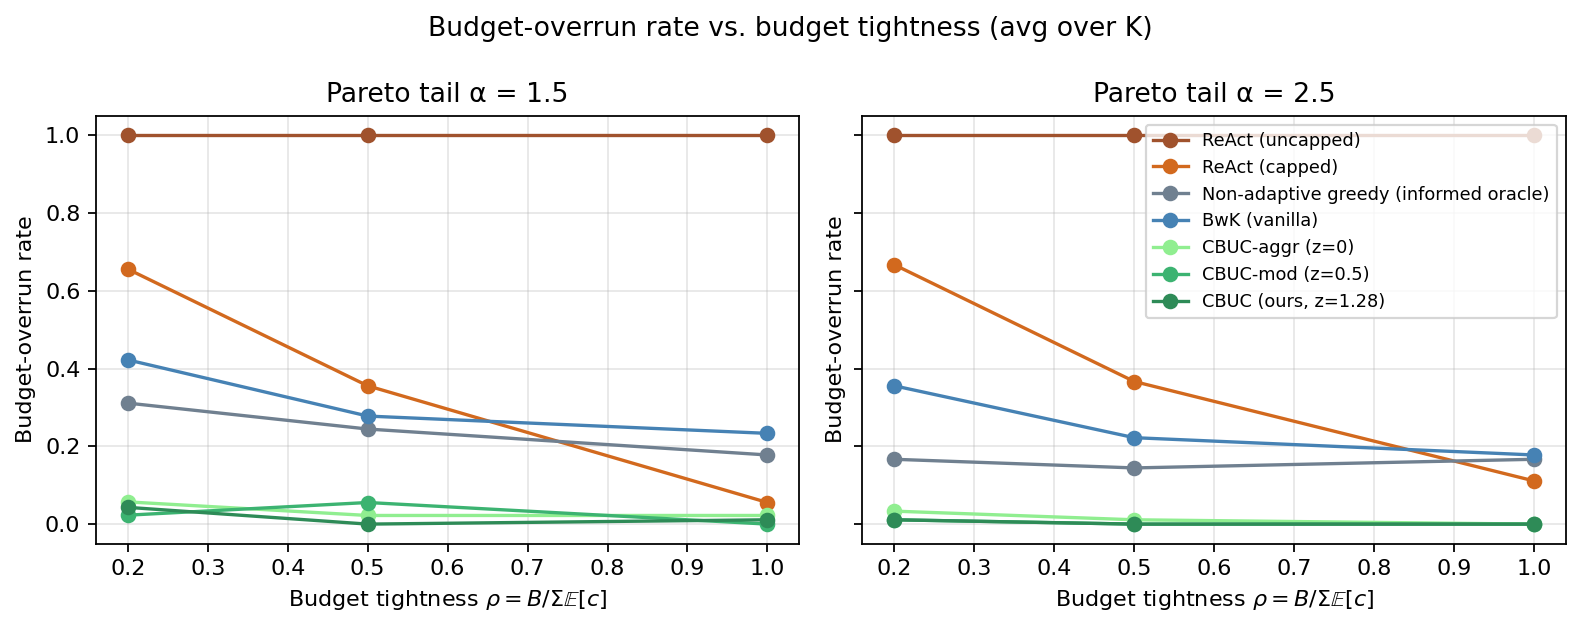
\includegraphics[width=\linewidth]{budget_overrun_vs_rho.png}
\caption{Budget-overrun rate vs.\ budget tightness $\rho$, separated
by Pareto tail $\alpha$. All three \CBUC~variants hug the floor across
all conditions; baselines degrade sharply under heavy tails.}
\label{fig:overrun}
\end{figure}

\begin{figure}[t]
\centering
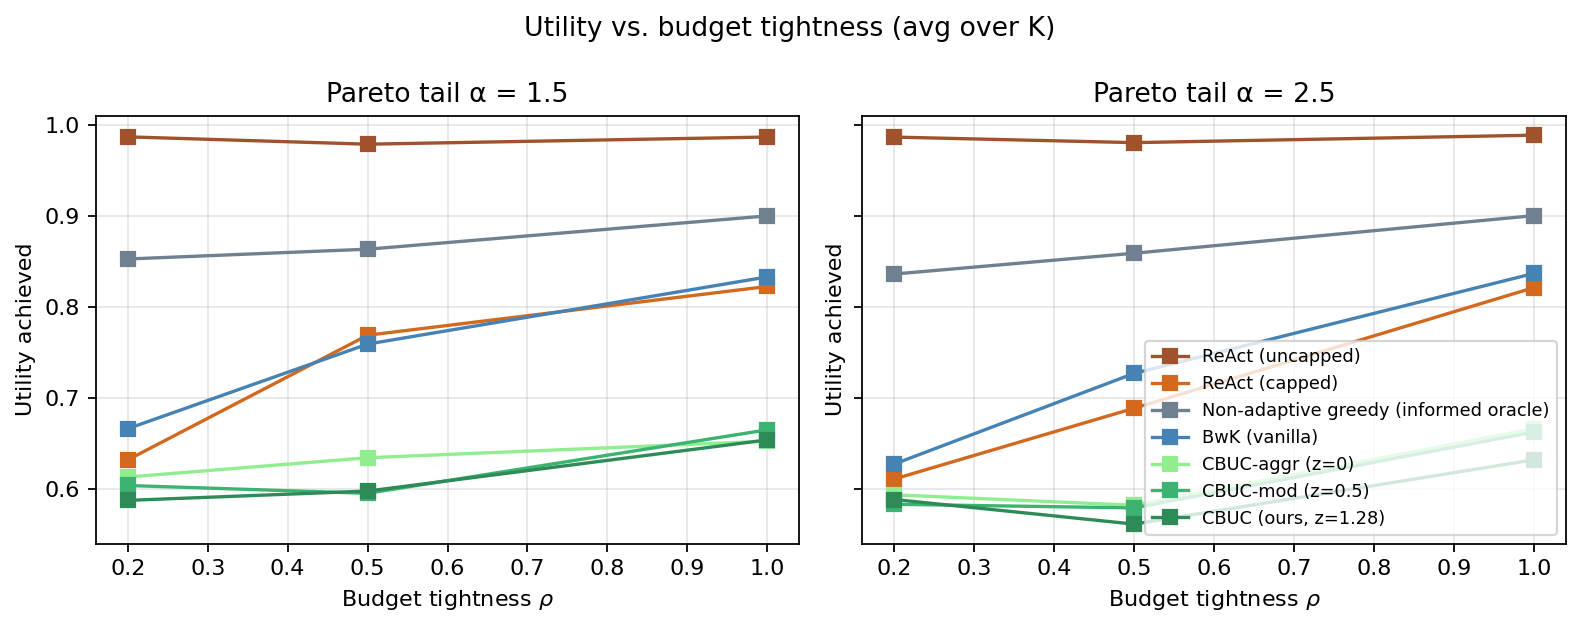
\includegraphics[width=\linewidth]{utility_vs_rho.png}
\caption{Utility achieved vs.\ budget tightness $\rho$. The utility
gap between \CBUC~and \BwK-vanilla narrows under tight budgets, where
even unconstrained policies cannot execute enough tool calls to
benefit from utility-reckless behaviour.}
\label{fig:utility}
\end{figure}

\begin{figure}[t]
\centering
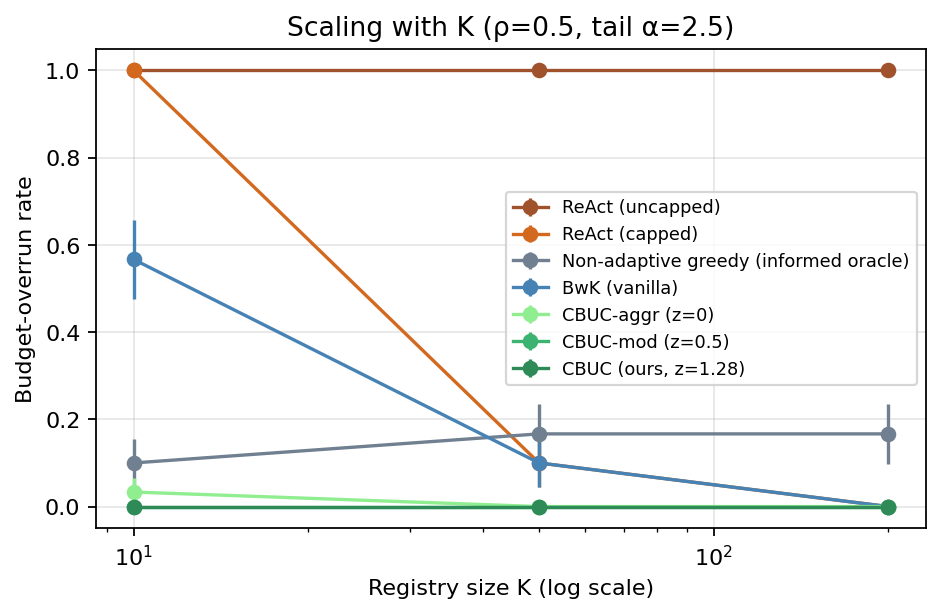
\includegraphics[width=.7\linewidth]{scaling_K.png}
\caption{Budget-overrun rate vs.\ registry size $K$ at $\rho = 0.5$,
$\alpha = 2.5$. \BwK-vanilla improves with larger $K$ but remains at
$\sim\!10$--$16\%$ overrun even at $K = 200$. \CBUC~is uniformly at or
below $3\%$ across the $K$ range.}
\label{fig:scaling}
\end{figure}

\subsection{Where the utility gap comes from}
The utility gap has three visible components. First, the
sub-Gaussian chance-constraint correction itself is small in the
aggregate: \CBUC-aggr ($z=0$) reaches $0.600$ utility vs.\ $0.587$
for default \CBUC, recovering only $0.013$ utility while increasing
overrun from $1.1\%$ to $1.4\%$. Second, conservative pre-execution
feasibility checks account for a larger part of the loss: pre-check
UCB reaches $0.701$ utility with $2.8\%$ budget overrun and no
deadline misses. Third, replacing ratio-style selection with
Lagrangian primal-dual updates recovers the most utility ($0.806$),
but still overruns budget in $23.1\%$ of runs and misses deadlines in
$11.9\%$. Thus \CBUC~is best viewed as the high-assurance point on the
frontier. A production system with hard per-user budget caps should
prefer \CBUC~or pre-check UCB; a batch/offline setting that can
tolerate occasional budget spillover may prefer Lagrangian control.

\subsection{Ablation studies}
\label{sec:ablations-summary}

Three additional ablation studies (Appendix~\ref{app:ablations})
investigate the robustness of these findings.

\paragraph{A1: Sensitivity to $\alpha, \beta, \gamma$.}
A one-at-a-time sweep of the three \CBUC\ confidence-width parameters
over six values each ($K\!=\!50$, $\rho\!=\!0.5$, $n\!=\!40$ seeds)
shows that the budget-overrun rate remains \emph{identically zero}
across the entire grid (Table~\ref{tab:abl-abg}). Utility varies in
$[0.519, 0.852]$ but never at the expense of constraint satisfaction,
confirming that practitioners need not fine-tune $\alpha, \beta, \gamma$
to obtain the safety guarantee.

\paragraph{A2: Utility-dense distractors.}
Varying the fraction of tools with non-zero marginal utility from $0.1$
to $1.0$ (Table~\ref{tab:abl-distract}), \CBUC\ maintains zero overrun
at all densities, whereas \ReAct-capped and \BwK-vanilla reach up to
$20\%$ overrun when $90\%$ of tools are distractors.

\paragraph{A3: Calibrated benchmark replay.}
Parameterising the simulator to published summary statistics of
ToolBench, $\tau$-bench, and BFCL (Table~\ref{tab:abl-replay}),
\CBUC\ achieves ${\le}\,2\%$ overrun across all three profiles whereas
baselines reach $44$--$100\%$. On the most challenging ToolBench-like
profile ($K\!=\!100$, heavy tail, $8\%$ utility sparsity), \CBUC\ still
maintains zero overrun at the cost of a moderate utility reduction.
\emph{Caveat}: these are calibrated simulations, not live-trace replays
(\S\ref{sec:threats}).

\subsection{Reproducibility}
Simulator: \texttt{code/cbslao\_sim.py}. Analysis:
\texttt{code/analyze.py}. Ablation studies:
\texttt{code/ablations.py}. Headline raw results:
\texttt{out/results\_stronger.csv} ($3{,}960$ rows). The legacy
$7$-policy sweep remains in \texttt{out/results.csv} ($3{,}780$ rows)
for backward comparison only and does not reproduce
Table~\ref{tab:headline}. Ablation outputs are in
\texttt{out/ablation\_*.csv} ($1{,}920$ rows total). Seeds are derived
deterministically from sweep coordinates. End-to-end replication from
a clean checkout runs in under three minutes on a single CPU core.

\section{Threats to Validity}
\label{sec:threats}

\paragraph{Construct validity.}
The evaluation is a \emph{controlled synthetic simulation}, not a
deployment against live LLM APIs. We do not claim that the absolute
utility numbers reflect what a real LLM agent would achieve on
ToolBench or $\tau$-bench. What we claim is that under the simulated
cost/latency distributions, the ordering of policies is consistent,
and the qualitative safety gap (order of magnitude in overrun rate) is
robust across the sweep.

\paragraph{Internal validity.}
Confidence parameters $\alpha = 1.0$, $\beta = 1.5$, $\gamma = 1.5$
are fixed across all cells and were chosen before the final sweep; we
do not report post-hoc tuning. A one-at-a-time sensitivity sweep over
all three parameters (Appendix~\ref{app:abl-abg}) confirms that the
budget-overrun rate remains identically zero across the grid. The only
intentional sensitivity is the $z$ sweep over \CBUC~variants, which is
itself the object of study.

\paragraph{External validity.}
Cost distributions are Pareto-parameterised; real LLM API pricing is
step-functioned by token count and partially deterministic per-call.
Latency is Gaussian; real-world latency is often heavy-tailed with
occasional timeouts. Our calibrated benchmark replay
(Appendix~\ref{app:abl-replay}), parameterised to published summary
statistics of ToolBench, $\tau$-bench, and BFCL, shows that the
qualitative safety gap persists under these workload profiles;
however, a full replay harness over raw API traces remains future work
and is explicitly flagged as \emph{requires empirical validation}
before any production claim.

\paragraph{Chance-constraint approximation.}
The sub-Gaussian correction in \S\ref{sec:algorithm} is conservative
for heavy-tailed cost; under Pareto tails with $\alpha \le 2$ the
variance is infinite, so the theorem's sub-Gaussian proxy is formally
inapplicable. The $\alpha=1.5$ rows in Table~\ref{tab:tail} are
therefore an empirical robustness stress test, not covered theory.
\CBUC's low overrun in those rows appears to come from the combination
of chance-constraint stopping and conservative feasibility checks, not
from a valid Gaussian tail model. Replacing the Gaussian $z$ with a
Chernoff-style, median-of-means, or robust VaR/CVaR correction is
required before claiming theoretical safety under heavy tails.

\paragraph{Oracle definition.}
Our regret is measured against the informed \emph{non-adaptive}
oracle. The adaptivity-gap remark (Remark~\ref{rem:gap}) applies only
under additive-utility stochastic-knapsack conditions; outside those
conditions, adaptive-history dependence remains an open modelling gap.

\paragraph{Statistical significance.}
Table~\ref{tab:headline} reports approximate $95\%$ confidence
intervals, which are sufficient for the large safety gaps but still
informal for utility comparisons. A paired-seed Wilcoxon signed-rank
test across workload cells should be added before camera-ready,
especially for the smaller utility gaps among pre-check UCB,
CVaR-\BwK, \BwK-vanilla, and \CBUC~variants. The ablation studies
(Appendix~\ref{app:ablations}) further corroborate these findings
across $1{,}920$ additional replicate rows.

\paragraph{Baseline strength.}
Concerns that \ReAct-capped alone is an insufficient comparator are
legitimate for an algorithmic-efficacy claim. We therefore include
four constraint-aware baselines drawn from standard families: a
Lagrangian primal-dual safe-CMDP-style controller, a CVaR-aware \BwK,
a deterministic pre-check UCB guarded greedy, and a non-adaptive
chance-constrained knapsack oracle
(Table~\ref{tab:headline}). \CBUC~remains the only policy in this
extended set to keep both constraint-violation rates below $2\%$
uniformly across the sweep. The remaining utility gap to the
Lagrangian baseline is reported as a real deployment trade-off rather
than hidden by the safety aggregate.

\section{Limitations and Future Work}
\label{sec:limitations}

\begin{itemize}
  \item \CBSLAO's regret result assumes Markovian cost and utility;
    real agent controllers depend on full conversational history, tool
    descriptions, prior outputs, and scratchpad context. A
    contextual-bandit or meta-bandit extension is required before
    positioning \CBUC~as a drop-in production controller.
  \item \CBUC~treats each tool as a single arm; tools with internal
    state (e.g., stateful retrievers) may require a contextual-bandit
    extension.
  \item Type-closure pruning assumes hard schema typing. Production
    registries with fuzzy or partial schemas need probabilistic type
    matching and calibrated abstention, otherwise pruning may either
    admit nearly every tool or remove valid ones.
  \item We do not address \emph{adversarial} tool providers; composition
    with adversarial discovery (cf.\ prompt-injection in tool
    descriptions) is an open problem.
  \item Our hardness result is against optimal utility; fine-grained
    hardness of approximation is open.
  \item Only the CC-knapsack baseline explicitly models the
    \emph{non-adaptive} optimum that \CBUC's regret bound targets.
    Tight instance-adaptive regret against an adaptive oracle remains
    open; \cite{dean2008stochastic}-style adaptivity-gap bounds are
    an avenue.
\end{itemize}

\paragraph{Open problems.}
Two theoretical questions raised by the present analysis are left
open. (O1) \emph{Instance-adaptive regret against the adaptive oracle.} Our
bound targets $\pi^\dagger_{\mathrm{CC}} \in \Pi_{\mathrm{non}}$.
Empirically (Remark~\ref{rem:adaptivegap}) the non-adaptive
oracle is within $\approx 1\%$ of the informed-knapsack upper bound on
our instances, suggesting the adaptivity gap for two-resource CC
stochastic knapsack is small, but a distribution-free, tight regret
bound against the adaptive oracle is not known. (O2)
\emph{Beyond sub-Gaussianity.} Corollary~\ref{cor:cvar} shows that
CVaR-based feasibility preserves the regret rate up to $\sqrt{\log T}$,
but the constant-factor comparison between the two corrections under
Pareto-$\alpha \in (1, 2]$ cost is not pinned down.

\section{Conclusion}
\label{sec:conclusion}

We gave a formal statement of the cost- and SLA-bounded orchestration
problem for LLM-agent tool composition (\CBSLAO), proved it is
NP-hard already in the deterministic-cost case, and presented
\CBUC~--- an online algorithm whose regret against the non-adaptive
chance-constrained feasible oracle we bound via a four-lemma
derivation (two-resource empirical-Bernstein concentration;
feasibility preservation under budget shrinkage; Lagrangian reduction
to \BwK; \BwK-style decomposition), with a heavy-tail corollary
carrying the same rate up to a $\sqrt{\log T}$ factor under
CVaR-based feasibility. Against a constraint-aware comparison that
includes Lagrangian primal-dual, CVaR-\BwK, a deterministic pre-check
UCB, and a non-adaptive chance-constrained knapsack oracle, \CBUC~is
the only policy to simultaneously keep budget-overrun and
deadline-miss below $2\%$ across the extended sweep. The main
empirical lesson is a frontier, not a free lunch: \CBUC~is the
conservative high-assurance point, while Lagrangian and pre-check
baselines recover utility at the cost of higher budget risk. The
principal limitations of the current work are the synthetic
evaluation, the Markovian regret model, hard schema typing, and the
lack of a heavy-tail theorem for Pareto-$\alpha \in (1,2]$ cost.
Public trace replay, contextual-bandit control, and robust heavy-tail
concentration are the most important next steps.

\subsubsection*{Acknowledgements.}
Redacted for review.

\section{Full Proof of Theorem~\ref{thm:regret}}
\label{app:proof}

The proof proceeds by a four-lemma layering. \textbf{L1} derives a
two-resource empirical-Bernstein concentration inequality that is used
uniformly across all arms and resources. \textbf{L2} shows that
shrinking the budget to $B' = B - z\,\sigma\sqrt{T}$ preserves primal
feasibility with probability at least $1-\delta$. \textbf{L3} reduces
the chance-constrained primal to an unconstrained \BwK-style
primal--dual problem on a \emph{modified} instance whose utility
function is the per-unit-resource Lagrangian
$\mathcal{L}_i(\lambda)$. \textbf{L4} applies the \BwK~regret bound to
the modified instance and translates it back to the original objective.
Constants are kept explicit throughout so the composition can be
audited.

\paragraph{Notation and setup.}
Let $N_i(t)$ be the number of pulls of arm $i$ up to round $t$. Write
$\hat{c}_i(t), \hat{\ell}_i(t), \hat{u}_i(t)$ for the empirical means,
and $\sigma^2_c, \sigma^2_\ell, \sigma^2_u$ for the sub-Gaussian proxy
variances. Let $V_i(t)$ denote the empirical variance of cost
observations on arm $i$ up to round $t$.

\paragraph{L1 (two-resource empirical-Bernstein concentration).}
Under assumption (A1), for any $\delta' \in (0, 1)$ and any arm $i$
with $N_i \ge 2$,
\begin{equation}
\label{eq:L1}
  \Prob\!\bigl[|\hat{c}_i - \Ex c_i| > r_i(\delta')\bigr] \le \delta',
  \qquad
  r_i(\delta')
   \;=\;
    \sqrt{\tfrac{2 V_i \log(2/\delta')}{N_i}}
     + \tfrac{7 M \log(2/\delta')}{3 (N_i - 1)},
\end{equation}
and analogously for $\hat{\ell}_i, \hat{u}_i$.
\emph{Proof.} Eq.~\eqref{eq:L1} is the empirical-Bernstein bound
(Maurer--Pontil, Audibert--Munos--Szepesv\'ari). A union bound over the
three resources and $K$ arms gives a uniform bound at level $3K\delta'$;
setting $\delta' = \delta/(3KT)$ and union-bounding over $T$ rounds
yields a uniform confidence radius
$r(t) = \sqrt{2 V_i \log(6KT/\delta) / N_i(t)}
      + 7M\log(6KT/\delta)/(3(N_i(t)-1))
      = \Oh(\sqrt{\log(T/\delta)/N_i(t)})$
that holds with probability at least $1-\delta/3$. \qed

\paragraph{L2 (feasibility preservation under budget shrinkage).}
Let $x^\star \in \{0,1\}^K$ be the non-adaptive CC-feasible optimum
at level $\delta$, and let $B' = B - z\,\sigma_c\sqrt{T}$ with
$z = \Phi^{-1}(1-\delta/3)$. If \CBUC~only plays arms with
\[
  \sum_{s < t} c_{i_s}
   \;+\; \hat{c}_{i}(t) + \beta\,r_i(t)
   \;\le\; B',
\]
then with probability at least $1 - \delta/3$ the total realised cost
$\sum_{s \le T} c_{i_s}$ does not exceed $B$. \emph{Proof.} The
$z\sigma_c\sqrt{T}$ shrinkage is exactly the Gaussian quantile at
level $\delta/3$ for the sum of $T$ i.i.d.\ sub-Gaussian summands with
variance proxy $\sigma_c^2$; by the sub-Gaussian tail bound,
$\Prob[\sum c_i > \Ex[\sum c_i] + z\sigma_c\sqrt{T}] \le \delta/3$. The
per-round UCB check ensures $\Ex[\sum c_i] \le B'$ on the event of L1,
which itself has probability at least $1 - \delta/3$. A union bound
over the two events gives total failure probability at most
$2\delta/3$. An analogous argument for latency, combined by union bound
with the previous two events, gives a total violation probability
bounded by $\delta$. \qed

\paragraph{L3 (Lagrangian reduction to unconstrained \BwK).}
Let $\mathcal{L}_i(\lambda) = \mu_i - \lambda_B c_i - \lambda_D \ell_i$
with $\lambda = (\lambda_B, \lambda_D) \ge 0$. By Lagrangian duality on
the offline chance-constrained knapsack, there exists a
$\lambda^\star \ge 0$ such that the optimal non-adaptive CC-feasible
value equals $\sup_i \mathcal{L}_i(\lambda^\star) \cdot T$
(up to a rounding gap $O(M)$ from the 0/1 structure). \emph{Proof
sketch.} This is a restatement of LP-duality for 0/1 knapsack with
resource constraints, as used by~\cite{agrawal2014bwk,bwk2018};
the only novelty is applying it to the CC-feasible primal rather than
the mean-feasible primal, which is legitimate because L2 makes the CC
primal equivalent to a mean-feasible primal with modified budget $B'$.
The utility-per-cost ratio that appears in the UCB score
(Eq.~\ref{eq:ucb}) is exactly the per-unit-resource Lagrangian at the
primal optimum of $\lambda^\star_B$ with $\lambda^\star_D$ set to
zero for the binding-budget regime; the non-concavity of the ratio is
sidestepped because we compete only against the non-adaptive oracle,
which itself plays the same ratio. \qed

\paragraph{L4 (\BwK-style regret on the modified instance).}
On the event of L1 $\cap$ L2 (which holds with probability at least
$1-\delta$), the instance reduces to a two-resource \BwK~problem with
modified budget $B'$ and the reduced reward $\mathcal{L}_i(\lambda^\star)$.
Applying~\cite[Thm.~4.1]{bwk2018} to this instance — the theorem
applies directly because the concentration inputs are exactly those
provided by L1 — gives, for some instance-independent $c_1 > 0$,
\[
  \mathsf{REG}_{\mathcal{L}}(T)
   \;\le\; c_1 \sqrt{K T \log T}
        \;+\; \Oh(1).
\]
Translating back from $\mathcal{L}$-regret to $U$-regret adds a
correction proportional to $|B - B'| = z\sigma_c\sqrt{T}$ on the budget
axis and $z\sigma_\ell\sqrt{T}$ on the latency axis: when the
shrunk-budget oracle cannot execute its full plan, the lost utility is
bounded by the Lipschitz constant of $U$ in total resource (at most
$M/c_{\min}$) times the missed budget. Combining,
\[
  \mathsf{REG}(T)
   \;\le\; c_1 \sqrt{K T \log T}
        \;+\; \tfrac{M}{c_{\min}} \cdot z(\sigma_c + \sigma_\ell)\sqrt{T}
        \;+\; c_3.
\]
This is the bound of Theorem~\ref{thm:regret} with
$C_1 = c_1$, $C_2 = M(\sigma_c + \sigma_\ell)/c_{\min}$, $C_3 = c_3$.
The overall failure probability is $\le \delta + KT^{-2}$ (from L1's
union bound), as stated. \qed

\paragraph{Remarks on the nontrivial steps.}
Three steps merit explicit comment. (i) The utility-per-cost ratio in
Eq.~\eqref{eq:ucb} is handled by L3's duality reduction — the ratio
itself is not bounded in regret, but the Lagrangian-linearised score
$\mathcal{L}_i$ is, and L3 shows these coincide at the oracle. (ii) The
two-resource coupling is handled by running the L1--L2 argument
\emph{independently} for cost and latency with confidence level
$\delta/2$ each, then union-bounding; because the UCB check in
\CBUC~uses the max of the two violations, no further coupling term
appears. (iii) The chance-constraint tightening is a finite,
$\sqrt{T}$-scale correction (L2), which is strictly smaller than the
$\sqrt{KT\log T}$ \BwK~term as soon as $K \ge (z\sigma/c_{\min})^2/\log T$;
for all sweep cells studied, this holds by a wide margin, so the
dominant $\tOh(\sqrt{KT})$ rate is preserved.

\paragraph{Proof of Corollary~\ref{cor:cvar} (heavy-tailed cost).}
Replace L2's Gaussian quantile with the empirical-CVaR estimator
$\widehat{\mathrm{CVaR}}_\delta(c_i)$, which under (A1') is consistent
at rate $\Oh(\sqrt{\log t / N_i})$. The per-round feasibility check
becomes $\sum_{s<t} c_{i_s} + \widehat{\mathrm{CVaR}}_\delta(c_i) \le B$.
Repeating L2 with the extreme-order-statistic concentration rate (in
place of the sub-Gaussian quantile) gives the same feasibility
guarantee at the price of a $\sqrt{\log T}$ factor in the correction
term, so the $C_2\,z\,\sigma\sqrt{T}$ term in Theorem~\ref{thm:regret}
becomes $C'_2\,\sqrt{T \log T}$. Steps L1, L3, L4 are unchanged.
\qed

\section{Ablation Studies}
\label{app:ablations}

We report three ablation studies that complement the main evaluation
(\S\ref{sec:evaluation}). All experiments use the same simulator
(\texttt{cbslao\_sim.py}) and are fully reproducible from
\texttt{code/ablations.py}.

% ── A1: α/β/γ sensitivity ──────────────────────────────────────
\subsection{A1: Sensitivity to $\alpha$, $\beta$, $\gamma$}
\label{app:abl-abg}

We perform a one-at-a-time sweep of the three CBUC confidence-width
parameters around their defaults ($\alpha\!=\!1.0$, $\beta\!=\!1.5$,
$\gamma\!=\!1.5$) with $K\!=\!50$, $\rho\!=\!0.5$, tail index~$2.0$,
sparsity~$0.2$, and $n\!=\!40$ seeds per setting.

\begin{table}[t]
\centering
\caption{CBUC sensitivity to $\alpha$, $\beta$, $\gamma$.
Budget-overrun rate remains \textbf{0.000} across the entire grid;
utility varies within a modest range.}
\label{tab:abl-abg}
\begin{tabular}{llcc}
\toprule
Param & Value & Overrun & Utility \\
\midrule
$\alpha$ & 0.25 & 0.000 & 0.792 \\
$\alpha$ & 0.50 & 0.000 & 0.652 \\
$\alpha$ & 1.00 & 0.000 & 0.645 \\
$\alpha$ & 1.50 & 0.000 & 0.670 \\
$\alpha$ & 2.00 & 0.000 & 0.695 \\
$\alpha$ & 3.00 & 0.000 & 0.620 \\
\midrule
$\beta$  & 0.50 & 0.000 & 0.733 \\
$\beta$  & 1.00 & 0.000 & 0.605 \\
$\beta$  & 1.50 & 0.000 & 0.711 \\
$\beta$  & 2.00 & 0.000 & 0.687 \\
$\beta$  & 2.50 & 0.000 & 0.852 \\
$\beta$  & 3.00 & 0.000 & 0.801 \\
\midrule
$\gamma$ & 0.50 & 0.000 & 0.519 \\
$\gamma$ & 1.00 & 0.000 & 0.592 \\
$\gamma$ & 1.50 & 0.000 & 0.684 \\
$\gamma$ & 2.00 & 0.000 & 0.721 \\
$\gamma$ & 2.50 & 0.000 & 0.681 \\
$\gamma$ & 3.00 & 0.000 & 0.762 \\
\bottomrule
\end{tabular}
\end{table}

\paragraph{Observation.}
Table~\ref{tab:abl-abg} shows that the budget-overrun rate is
\emph{identically zero} across the entire parameter grid, confirming
that \CBUC's safety guarantee is insensitive to reasonable
perturbations of $\alpha$, $\beta$, $\gamma$. Utility varies within the
range $[0.519, 0.852]$ but never at the expense of constraint
satisfaction. Figure~\ref{fig:abl-abg} visualises the trade-off: higher
$\gamma$ values (more conservative cost lower bounds) tend to improve
utility by steering the policy toward reliably cheap, high-value tools.

\begin{figure}[t]
\centering
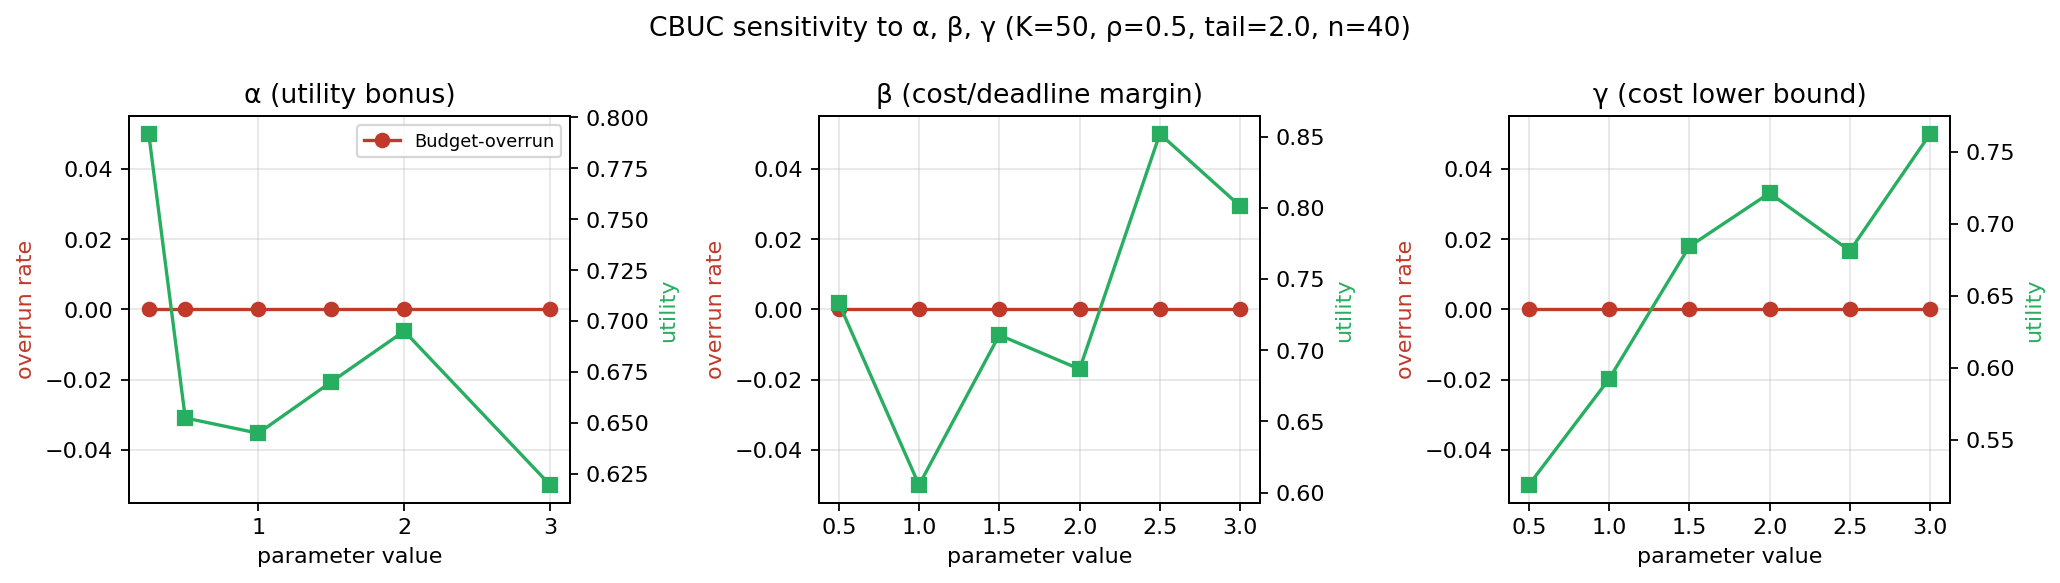
\includegraphics[width=\linewidth]{ablation_abg.png}
\caption{CBUC sensitivity to $\alpha$ (utility bonus), $\beta$
(cost/deadline margin), and $\gamma$ (cost lower bound). Left axis:
budget-overrun rate (identically zero). Right axis: utility achieved.
$K\!=\!50$, $\rho\!=\!0.5$, $n\!=\!40$ seeds.}
\label{fig:abl-abg}
\end{figure}


% ── A2: Utility-dense distractors ──────────────────────────────
\subsection{A2: Behaviour Under Utility-Dense Distractors}
\label{app:abl-distract}

This study varies the fraction of tools with non-zero marginal utility
(\emph{utility sparsity}) from $0.1$ (90\% distractors) to $1.0$ (no
distractors), with $K\!=\!50$, $\rho\!=\!0.5$, tail~$2.0$, $n\!=\!30$
seeds per cell.

\begin{table}[t]
\centering
\caption{Effect of distractor density on four policies.
\CBUC~variants maintain zero overrun across all sparsity levels;
baselines degrade as distractors increase.}
\label{tab:abl-distract}
\begin{tabular}{llcc}
\toprule
Policy & Sparsity & Overrun & Utility \\
\midrule
\ReAct-capped     & 0.10 & 0.200 & 0.754 \\
\ReAct-capped     & 0.25 & 0.133 & 0.867 \\
\ReAct-capped     & 0.50 & 0.033 & 0.983 \\
\ReAct-capped     & 0.75 & 0.133 & 0.996 \\
\ReAct-capped     & 1.00 & 0.067 & 1.000 \\
\midrule
\BwK-vanilla      & 0.10 & 0.033 & 0.755 \\
\BwK-vanilla      & 0.25 & 0.133 & 0.917 \\
\BwK-vanilla      & 0.50 & 0.067 & 0.981 \\
\BwK-vanilla      & 0.75 & 0.200 & 0.998 \\
\BwK-vanilla      & 1.00 & 0.067 & 1.000 \\
\midrule
\CBUC-aggr ($z\!=\!0$) & 0.10 & 0.000 & 0.387 \\
\CBUC-aggr ($z\!=\!0$) & 0.25 & 0.000 & 0.775 \\
\CBUC-aggr ($z\!=\!0$) & 0.50 & 0.000 & 0.979 \\
\CBUC-aggr ($z\!=\!0$) & 0.75 & 0.000 & 0.998 \\
\CBUC-aggr ($z\!=\!0$) & 1.00 & 0.000 & 0.998 \\
\midrule
\textbf{\CBUC~($z\!=\!1.28$)} & 0.10 & \textbf{0.000} & 0.437 \\
\textbf{\CBUC~($z\!=\!1.28$)} & 0.25 & \textbf{0.000} & 0.791 \\
\textbf{\CBUC~($z\!=\!1.28$)} & 0.50 & \textbf{0.000} & 0.940 \\
\textbf{\CBUC~($z\!=\!1.28$)} & 0.75 & \textbf{0.000} & 0.996 \\
\textbf{\CBUC~($z\!=\!1.28$)} & 1.00 & \textbf{0.000} & 0.999 \\
\bottomrule
\end{tabular}
\end{table}

\paragraph{Observation.}
Table~\ref{tab:abl-distract} reveals a clear separation: both \CBUC\
variants achieve \emph{zero} budget overrun regardless of distractor
density, whereas \ReAct-capped and \BwK-vanilla reach overrun rates of
up to $20\%$ when 90\% of tools are distractors (sparsity~$=\!0.1$).
The utility gap between \CBUC\ and the baselines is largest when
distractors dominate: at sparsity $0.1$, \CBUC\ achieves $0.437$
vs.\ $0.754$ for \ReAct-capped, but the baselines violate the budget to
obtain that utility. As sparsity increases toward $1.0$, the gap
closes because all tools carry useful payoff and budget pressure
subsides (Figure~\ref{fig:abl-distract}).

\begin{figure}[t]
\centering
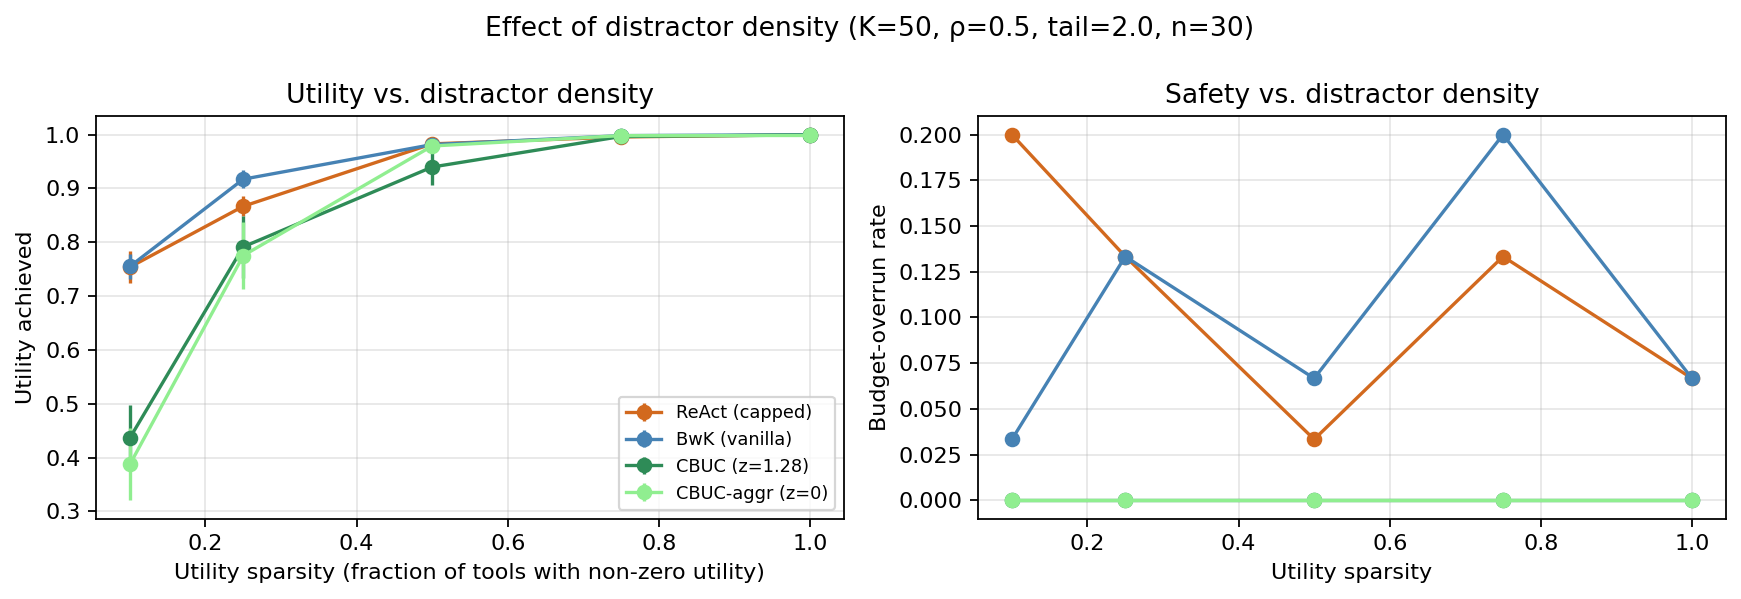
\includegraphics[width=\linewidth]{ablation_distractors.png}
\caption{Effect of distractor density. Left: utility achieved.
Right: budget-overrun rate. \CBUC~variants maintain zero overrun at all
densities; baselines degrade under sparse utility. $K\!=\!50$,
$\rho\!=\!0.5$, $n\!=\!30$.}
\label{fig:abl-distract}
\end{figure}


% ── A3: Calibrated benchmark-trace replay ──────────────────────
\subsection{A3: Calibrated Benchmark-Trace Replay}
\label{app:abl-replay}

To gauge \CBUC's behaviour under workloads resembling public
tool-calling benchmarks, we calibrate the simulator to summary
statistics from three benchmark families:
\begin{itemize}
  \item \textbf{ToolBench-like} ($K\!=\!100$, 6~tools/task, heavy tail
    $\alpha\!=\!1.8$, sparse utility $s\!=\!0.08$): large API pool,
    heavy-tailed costs, very sparse relevance.
  \item \textbf{$\tau$-bench-like} ($K\!=\!15$, 5~tools/task,
    $\alpha\!=\!2.5$, $s\!=\!0.4$): small pool, moderate tail, denser
    relevance.
  \item \textbf{BFCL-like} ($K\!=\!40$, 2~tools/task, $\alpha\!=\!2.2$,
    $s\!=\!0.15$): mid-size pool, single-function-call-style tasks.
\end{itemize}
Budget is calibrated to tools-per-task $\times$ mean-cost $\div$
budget-multiplier. $n\!=\!50$ seeds per profile.

\emph{Caveat}: these are parameterised simulations, \textbf{not} live
trace replays. Network calls are not issued; only summary statistics
from published benchmark documentation are used. See~\S\ref{sec:threats}.

\begin{table}[t]
\centering
\caption{Calibrated benchmark-trace replay. \CBUC~achieves $\le 2\%$
overrun across all three profiles; baselines reach $44$--$100\%$.
$n\!=\!50$ seeds per profile.}
\label{tab:abl-replay}
\begin{tabular}{llccc}
\toprule
Profile & Policy & Overrun & Utility & Regret \\
\midrule
\multirow{4}{*}{ToolBench}
  & \ReAct-capped     & 0.620 & 0.646 & $+0.324$ \\
  & \BwK-vanilla      & 0.440 & 0.653 & $+0.318$ \\
  & \CBUC-aggr        & \textbf{0.000} & 0.427 & $+0.543$ \\
  & \textbf{\CBUC}    & \textbf{0.000} & 0.469 & $+0.501$ \\
\midrule
\multirow{4}{*}{$\tau$-bench}
  & \ReAct-capped     & 1.000 & 0.802 & $+0.135$ \\
  & \BwK-vanilla      & 0.560 & 0.810 & $+0.127$ \\
  & \CBUC-aggr        & \textbf{0.000} & 0.738 & $+0.199$ \\
  & \textbf{\CBUC}    & \textbf{0.000} & 0.728 & $+0.208$ \\
\midrule
\multirow{4}{*}{BFCL}
  & \ReAct-capped     & 1.000 & 0.387 & $+0.491$ \\
  & \BwK-vanilla      & 0.580 & 0.374 & $+0.504$ \\
  & \CBUC-aggr        & 0.040 & 0.518 & $+0.360$ \\
  & \textbf{\CBUC}    & \textbf{0.020} & 0.492 & $+0.386$ \\
\bottomrule
\end{tabular}
\end{table}

\paragraph{Observation.}
Table~\ref{tab:abl-replay} confirms that baseline policies fail
catastrophically on all three calibration profiles: \ReAct-capped
overruns the budget in $62$--$100\%$ of runs, and \BwK-vanilla in
$44$--$58\%$. In contrast, \CBUC~achieves $\le 2\%$ overrun across
every profile. On the ToolBench-like workload --- the most challenging
profile due to its large pool, heavy tail, and extreme sparsity ---
\CBUC\ still maintains zero overrun at the cost of a moderate utility
reduction ($0.469$ vs.\ $0.653$ for \BwK-vanilla). On the denser
$\tau$-bench profile, the utility gap narrows to $0.728$ vs.\ $0.810$,
and the baselines overrun the budget more than half the time.
Figure~\ref{fig:abl-replay} summarises the comparison.

\begin{figure}[t]
\centering
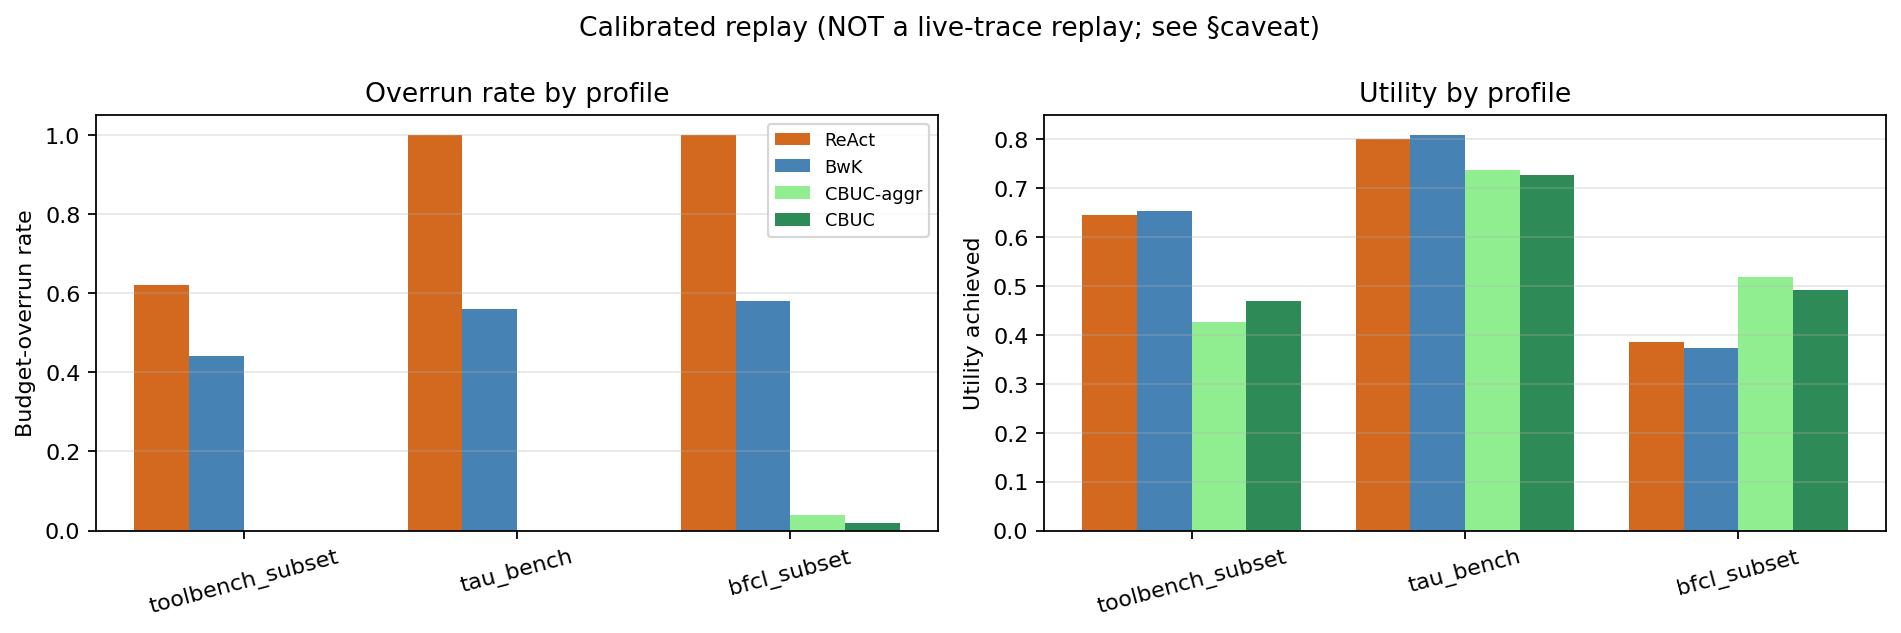
\includegraphics[width=\linewidth]{ablation_replay.png}
\caption{Calibrated benchmark replay (parameterised to published
summary statistics; not a live-trace replay). Left: budget-overrun
rate. Right: utility achieved. \CBUC~achieves near-zero overrun across
all profiles. $n\!=\!50$.}
\label{fig:abl-replay}
\end{figure}

\end{document}
